\documentclass[a4paper,10pt]{article}
\usepackage[left=1in, right=1in, top=1in, bottom=0.8in]{geometry}
\usepackage{titlesec, xcolor, enumitem, hyperref, graphicx, tcolorbox, fontspec, multicol, setspace}
\usepackage{tikz}
\usepackage{ragged2e}
\usepackage{fontawesome5}
\usepackage{array, tabularx, colortbl}

% Set main font
\setmainfont{Noto Sans}[
    Kerning = On,
    Numbers = Uppercase, 
    BoldFont = Noto Sans SemiBold
]

% Formatting settings
\setlength\parindent{0pt}
\setstretch{1.3}
\setlength\columnsep{0.25in}
\pagestyle{empty}

% Define custom colors
\definecolor{primary}{HTML}{6D7B8D}  % Muted blue-gray
\definecolor{secondary}{HTML}{B0BEC5} % Soft gray-blue
\definecolor{textcolor}{HTML}{37474F} % Deep gray
\definecolor{background}{HTML}{ECEFF1} % Light grayish background

% Title format
\titleformat{\section}{\large\bfseries\color{primary}}{}{0em}{}[\titlerule]

% Hyperlink setup
\hypersetup{
    colorlinks=true,
    linkcolor=primary,
    urlcolor=primary,
}

% Custom Box Design
\tcbset{
    sharp corners,
    colback = white,
    before skip = 0.2cm,
    after skip = 0.5cm
}

% Profile Box
\newtcolorbox{boxM}{
    fontupper = \color{white},
    rounded corners,
    arc = 6pt,
    colback = primary, 
    colframe = primary, 
    boxrule = 0pt, 
    bottomrule = 4.5pt,
    enhanced
}

\newtcolorbox{boxB}{
    boxrule = 1.5pt,
    colframe = primary,
    rounded corners,
    arc = 5pt   % corners roundness
}

% Project Box
\newtcolorbox{projectbox}[2][]{colback=secondary!20!white, colframe=secondary!80!black, title=#2, fonttitle=\bfseries, coltitle=black}

\begin{document}

% Header
\begin{minipage}{0.70\textwidth}
    {\LARGE\bfseries Sudipta Singha Rathi}\\[0.5em]
    {\large Software Developer | Distro Hopper | DevOps}\\[0.5em]
    \faPhone \ +8801746-579065 \quad
    \faGlobe \ \href{https://sudiptarathi2020.github.io}{sudiptarathi2020.github.io}\\
    \faEnvelope \ \href{mailto:jucse29.408@gmail.com}{jucse29.408@gmail.com} 
    \faGithub \ \href{https://github.com/sudiptarathi2020}{sudiptarathi2020}
    \faLinkedin \ \href{https://www.linkedin.com/in/sudiptarathi/}{sudiptarathi} \quad
    
\end{minipage}%
\hfill
\begin{minipage}{0.30\textwidth}
    \raggedleft
    \begin{tikzpicture}
        \clip [rounded corners=0.5cm] (0,0) rectangle (3cm,3cm);
        \node at (1.5cm,1.5cm) {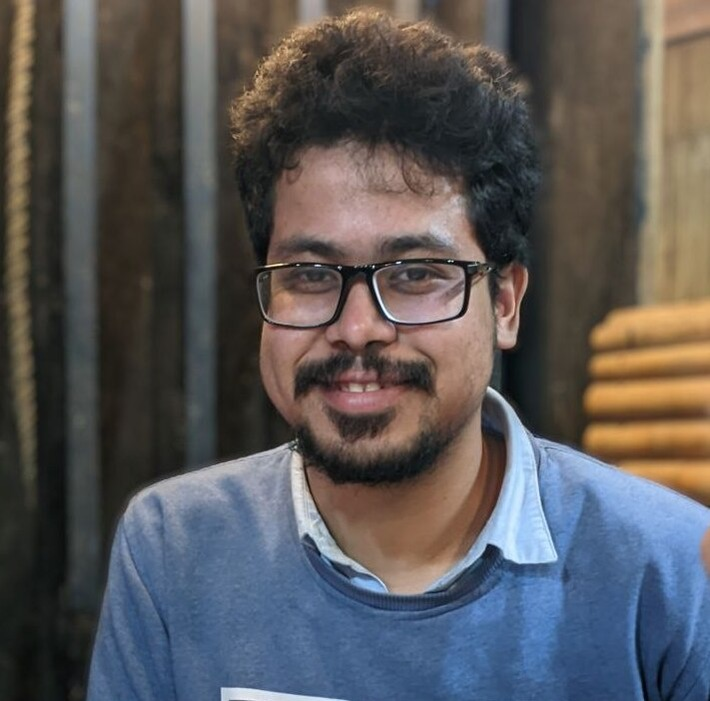
\includegraphics[width=3cm, height=3cm]{resources/profile.jpg}};
    \end{tikzpicture}
\end{minipage}

\vspace{1em}

% About Me
\section*{About Me}
A final year Computer Science and Engineering student at Jahangirnagar University, passionate about Machine Learning, Reinforcement Learning, System Design, Computer Security, Competative programming and DevOps.

% Education
\section*{Education}
\begin{itemize}[leftmargin=0.5cm]
    \item \textbf{Jahangirnagar University} – BSc in Computer Science and Engineering
    \item \textbf{Milestone College} – HSC in Science
    \item \textbf{Tetaigaon Rashid Uddin High School} – SSC in Science
\end{itemize}

% Skills
\section*{Skills}

\begin{table}[h!]
    \centering
    \renewcommand{\arraystretch}{1.4} % Increase row height for better readability
    \setlength{\arrayrulewidth}{1pt} % Increase border thickness

    \begin{tabularx}{\textwidth}{|>{\raggedright\arraybackslash}m{3cm}|>{\raggedright\arraybackslash}X|}
        \hline
        \rowcolor{primary} \textbf{\color{white} Category} & \textbf{\color{white} Skills} \\
        \hline
        \rowcolor{background} Programming & Python, C, C++, Java, LaTeX, Bash \\
        \hline
        Frameworks & Django \\
        \hline
        \rowcolor{background} Tools & Linux, Git, WSL, Docker, AWS \\
        \hline
        Databases & SQLite \\
        \hline
    \end{tabularx}
\end{table}
% Experience
\section*{Experience}
\begin{itemize}[leftmargin=0.5cm]
    \item \textbf{Technical Team Leader} – National Collegiate Programming Contest 2023, Jahangirnagar University
    \begin{itemize}
        \item Led the technical team in organizing and managing the programming contest.
        \item Coordinated technical aspects including setting up contest environment, installing ubuntu in almost 200 computers, monitoring.
    \end{itemize}
    \item \textbf{Mentor} – Jahangirnagar University Programming Community
    \begin{itemize}
        \item Actively mentor junior members in competitive programming.
        \item Provide guidance and training for improving problem-solving skills.
    \end{itemize}
\end{itemize}


% Projects
\section*{Projects}
\href{https://github.com/sudiptarathi2020/JUMCMS-Jahangirnagar-University-Medical-Center-Management-System.git}{\textbf{JUMCMS}}
\begin{boxB}
    To improve medical center operations, JUMCMS (Jahangirnagar University Medical Center Management System) is a web application built with Django. For Admins, Doctors, Patients, Lab technicians, and Store managers, it provides functionality tailored to their roles. Prescription management, test reporting, inventory control, and appointment scheduling are all made easier by the system.\\
    \href{https://github.com/sudiptarathi2020/JUMCMS-Jahangirnagar-University-Medical-Center-Management-System.git}{https://github.com/sudiptarathi2020/JUMCMS-Jahangirnagar-University-Medical-Center-Management-System.git}
\end{boxB}

\href{https://github.com/sudiptarathi2020/Software-Engineering-Lab-CSE404-Reports.git}{\textbf{Software Engineering Lab Reports}}
\begin{boxB}
    My collection of software engineering lab reports documenting various projects and experiments I did for CSE-404 Software Engineering Lab.\\
    \href{https://github.com/sudiptarathi2020/Software-Engineering-Lab-CSE404-Reports.git}{https://github.com/sudiptarathi2020/Software-Engineering-Lab-CSE404-Reports.git}
\end{boxB}

\href{https://github.com/sudiptarathi2020/Data-structures-and-Algorithms}{\textbf{Data Structure and Algorithms}}
\begin{boxB}
    My Data structure and algorithms template and codes. This repository contains cpp and python implementation for segment tree, binary index tree, red-black tree, avl tree, splay tree, treap, scc, centroid decomposition,convex hull, minheap and maxheap, heavy-light decomposition, huffman coding, line sweep, lowest common ancestor, sparse table, kd tree etc.\\ \href{https://github.com/sudiptarathi2020/Data-structures-and-Algorithms}{https://github.com/sudiptarathi2020/Data-structures-and-Algorithms}
\end{boxB}

\href{https://github.com/sudiptarathi2020/Simple-Chess-Engine.git}{\textbf{Chess Engine}}
\begin{boxB}
   This is a very simple chess game developed for my research project Reinforcement learning. This version will include minimax algorithm with alpha beta pruning for the engine part. Later version will be implemented using Monte Carlo Tree Search(MCTS).\\ \href{https://github.com/sudiptarathi2020/Simple-Chess-Engine.git}{https://github.com/sudiptarathi2020/Simple-Chess-Engine.git}
\end{boxB}

\href{https://github.com/sudiptarathi2020/puddle}{\textbf{Puddle}}
\begin{boxB}
    Simple E-commerce website for buying, selling toys and other goods. This django + template based web app is created following a youtube tutorial.\\  \href{https://github.com/sudiptarathi2020/puddle}{https://github.com/sudiptarathi2020/puddle}
\end{boxB}

\href{https://github.com/sudiptarathi2020/Digital-Image-Processing-Lab}{\textbf{DIP Lab Works}}
\begin{boxB}
    This repository contains a collection of Python scripts implementing various image processing techniques. These techniques are commonly used for detecting shapes, filtering noise, and transforming image color spaces. Each script includes a sample implementation along with detailed comments to help understand how each method works.\\ \href{https://github.com/sudiptarathi2020/Digital-Image-Processing-Lab}{https://github.com/sudiptarathi2020/Digital-Image-Processing-Lab}
\end{boxB}

\href{https://github.com/sudiptarathi2020/academic-report-maker.git}{\textbf{Academic Report Maker}}
\begin{boxB}
    A Django + React web application for generating academic reports with structured formatting.\\  \href{https://github.com/sudiptarathi2020/academic-report-maker.git}{https://github.com/sudiptarathi2020/academic-report-maker.git}
\end{boxB}

\href{https://github.com/sudiptarathi2020/Problem-Solves.git}{\textbf{Online Judge Problem Solutions}}
\begin{boxB}
    Solutions to problems from Codeforces, LightOJ, and other online judges, with explanations.  \href{https://github.com/sudiptarathi2020/Problem-Solves.git}{https://github.com/sudiptarathi2020/Problem-Solves.git}
\end{boxB}

\href{https://github.com/sudiptarathi2020/problem-tutorials}{\textbf{Lightoj Problem Tutorials}}
\begin{boxB}
    I contributed to this public repository for tutorial for various problems.  \href{https://github.com/sudiptarathi2020/problem-tutorials}{https://github.com/sudiptarathi2020/problem-tutorials}
\end{boxB}



% Online Judge Statistics
\section*{Online Judge Statistics}
\begin{multicols}{2}
\textbf{Codeforces:} 383 problems solved \\
\textbf{LightOJ:} 82 problems solved \\
\textbf{CSES} 53 problems solved \\
\textbf{Hackerearth} 23 problems solved
\end{multicols}

\end{document}
